\chapter{套筒}
\begin{figure}[htbp]
\centering
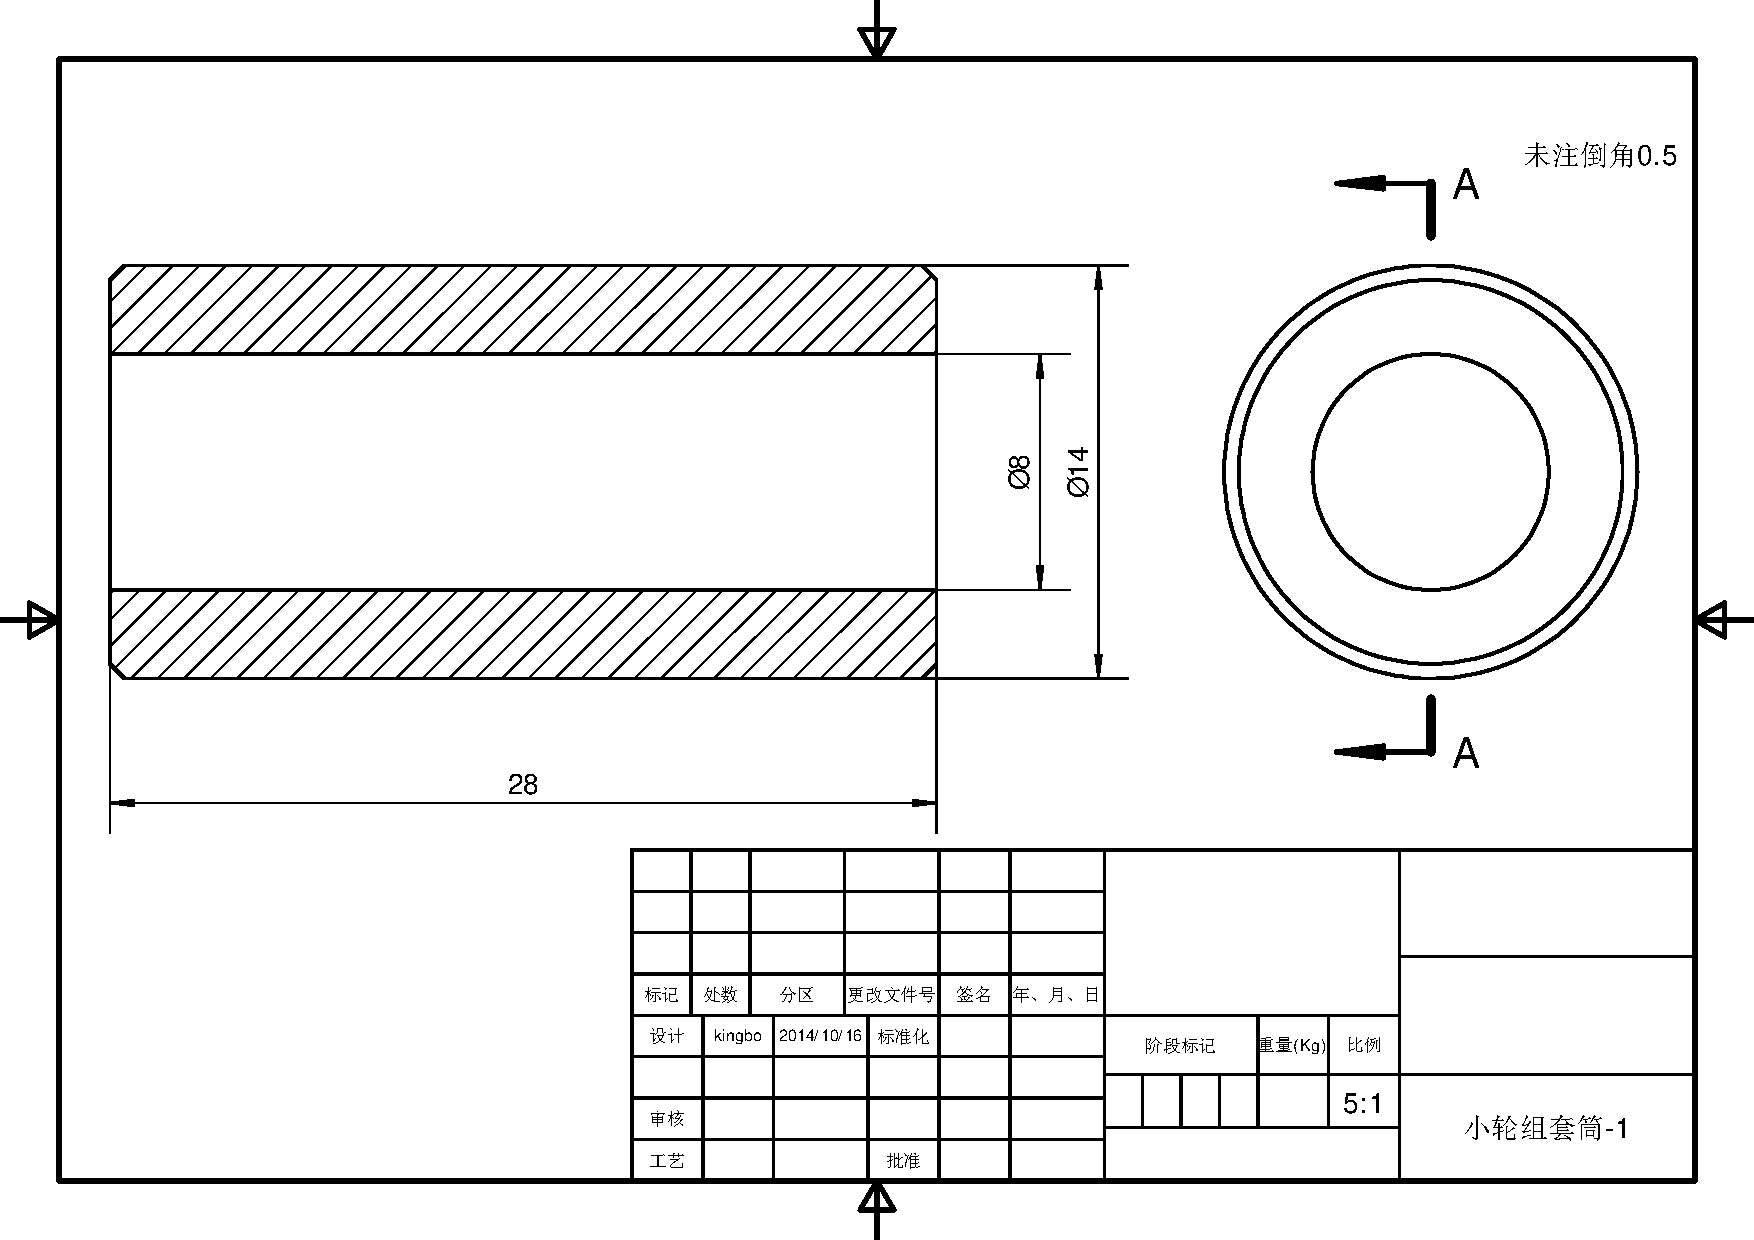
\includegraphics[scale=0.45]{xiaoluntaotong.pdf}
\caption{套筒零件图}\label{fig:xiaoluntaotong}
\end{figure}
%AutoCAD作为国际上广泛使用的流行的绘图工具,它具有较强的二维绘图和三维绘图功能,欢迎来到AutoCAD的三维世界,
本章我们的目标是用AutoCAD制作图\ref{fig:xiaoluntaotong}所示的小轮组构成零件轮轴的三维模型,并以此展开我们的AutoCAD三维建模之旅。本章将讲述以下内容:
\begin{itemize}
	\item 零件图的组成
	\item 圆柱体的构建
	\item 差集操作
	\item 倒角操作
	\item 视图的切换
	\item 三视图的形成
\end{itemize}

\endinput